%!TEX program = xelatex
%%%%%%%%%%%%%%%%%%%%%%%这是导言部分的开始%%%%%%%%

%========= 导言部分声明文档的类型=================
\documentclass{article}

	%=========导言部分可可以加载宏包=================
	\usepackage{amsmath}                % 数学公式排版宏包
	\usepackage{amssymb}                % 数学符号命令宏包
	\usepackage{amsthm}                 % 数学定理宏包
	\usepackage[UTF8]{ctex}             % 中文输入宏包
	\usepackage[a4paper]{geometry}      % 页面设置宏包
	\usepackage{setspace}               % 行间距宏包
	\usepackage{graphicx}               % 图片宏包
	\usepackage{listings}               % 代码宏包
	\usepackage{color}					% 颜色宏包
	\usepackage{xcolor}                 % 颜色处理宏包
	\usepackage{float}                  % 浮动对象式样宏包
	\usepackage{fontspec}
	\usepackage{enumerate}				% 列举编号包
	
	%=========页面设置==============================
	\geometry{left=1cm,right=1cm,top=1cm,bottom=2cm}
	\onehalfspacing
	\setlength\parindent{0em}

	%=========代码格式设置============================
	\definecolor{dkgreen}{rgb}{0,0.6,0}
	\definecolor{gray}{rgb}{0.5,0.5,0.5}
	\definecolor{mauve}{rgb}{0.58,0,0.82}
	% \setmonofont{Consolas}
	\lstset{
		numbers = left, 	
		numberstyle = \color{gray}, 
		keywordstyle = \color{blue},
		commentstyle = \color{dkgreen}, 
		stringstyle = \color{mauve},
		basicstyle = \ttfamily,
		breaklines = true,
		frame = shadowbox, % 阴影效果
		rulesepcolor = \color{ red!20!green!20!blue!20} ,
		escapeinside = ``, % 英文分号中可写入中文
		xleftmargin = 2em,xrightmargin=2em, aboveskip=1em,
		framexleftmargin = 2em
	} 

%=========导言部分可以定义标题信息===============
\title{组会报告}
\author{徐益}
\date{\today}
%%%%%%%%%%%%%%%%%%%%%%%这是导言部分的结束%%%%%%%%%

%%%%%%%%%%%%%%%%%%%%%%%这是正文部分的开始%%%%%%%%%
\begin{document}

%=========生成标题================================
\maketitle

%=========开始正文的输入==========================

%===========第一节=================
\section{工作内容}
1. 学习High-Throughput Multi-Core LDPC Decoders Based on x86 Processor。

2. 学习相关代码。

%===========第一节=================
\section{论文对layered-ms算法的改进}
\subsection{原数据结构}
\begin{figure}[H]
	\centering
	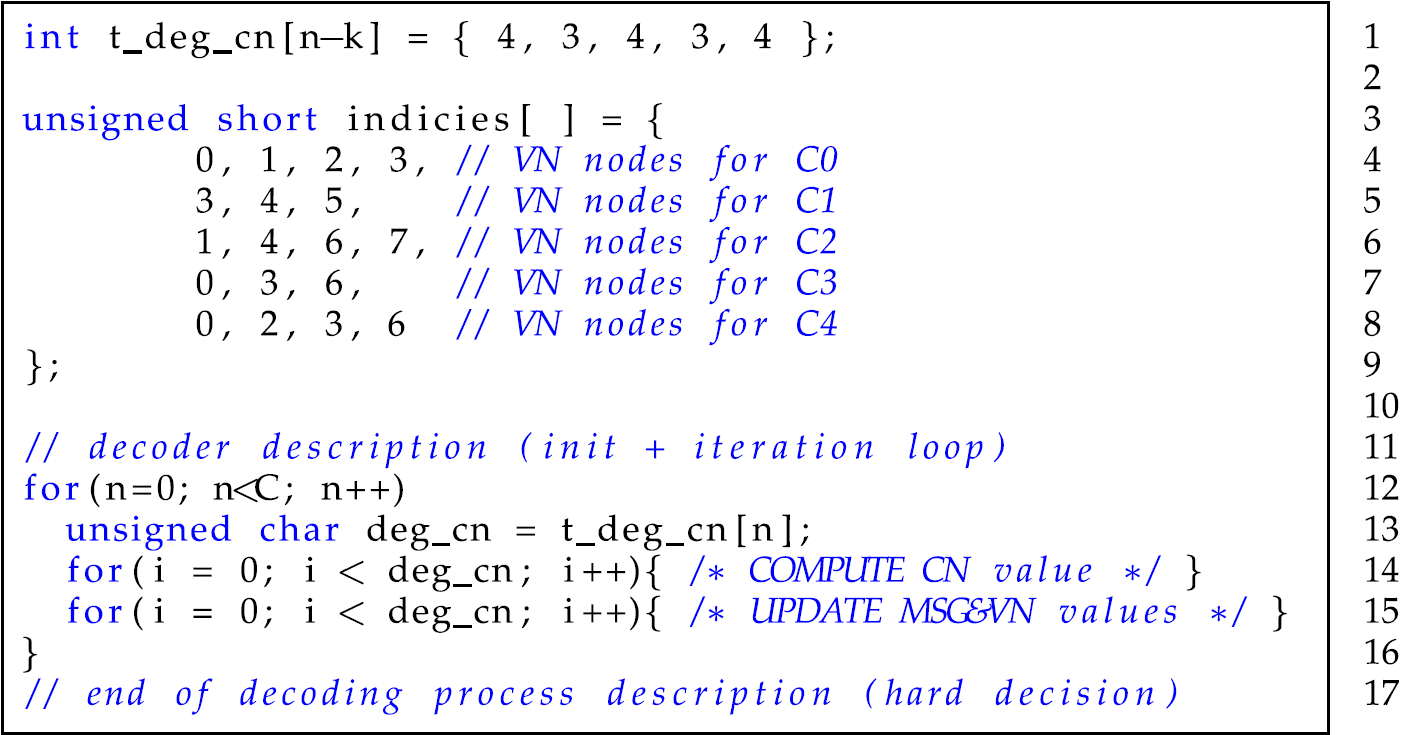
\includegraphics[width = .8\textwidth]{kernel.png}
	\caption{Naive decoder kernel description using constant arrays}
\end{figure}
空间占用情况:
\begin{equation}
	\Delta = 4 \times n + 4 \times m + 2 \times m + (n-k).
\end{equation}
\subsection{msg类型优化}
从float变成int8\_t\\
空间占用情况:
\begin{equation}
	\Delta = n + m + 2 \times m + (n-k).
\end{equation}
\subsection{基于交织的并行计算}
\begin{figure}[H]
	\centering
	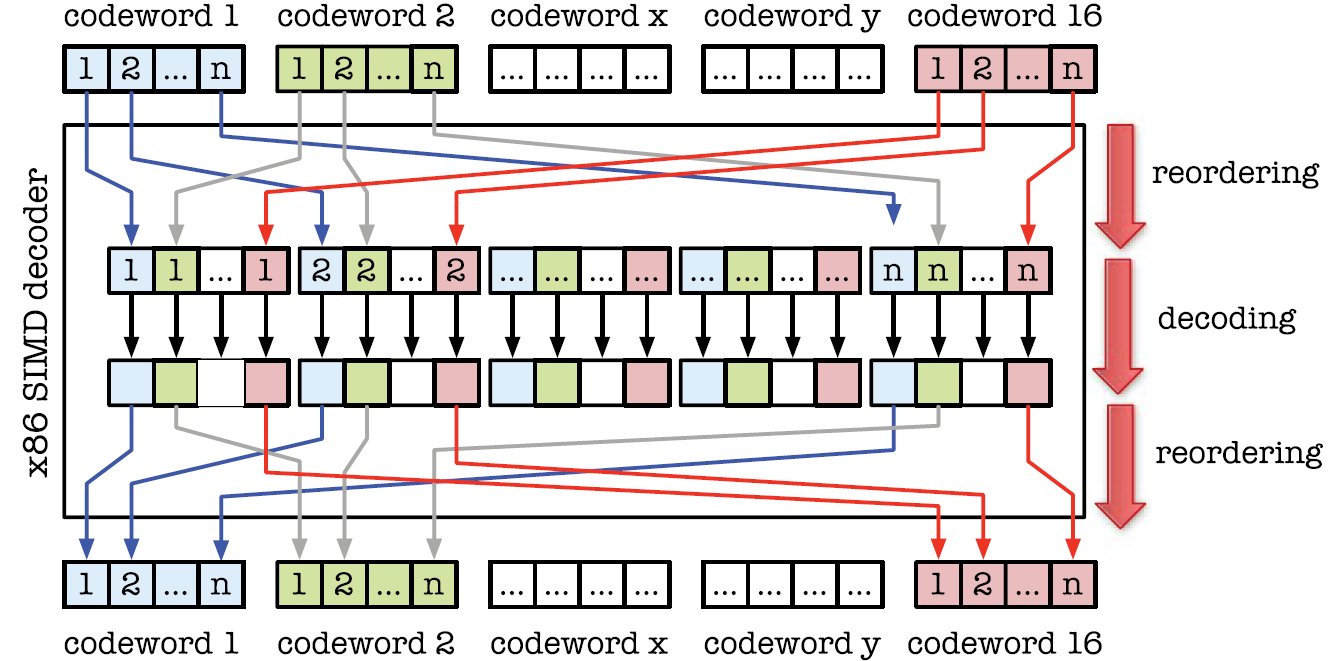
\includegraphics[width = .8\textwidth]{inter.png}
	\caption{Data interleaving and desinterleaving processes}
\end{figure}
空间占用情况:
\begin{equation}
	\Delta = q \times n + q \times m + 2 \times m + (n-k).
\end{equation}
\subsection{重新排布校验矩阵}
\begin{figure}[H]
	\centering
	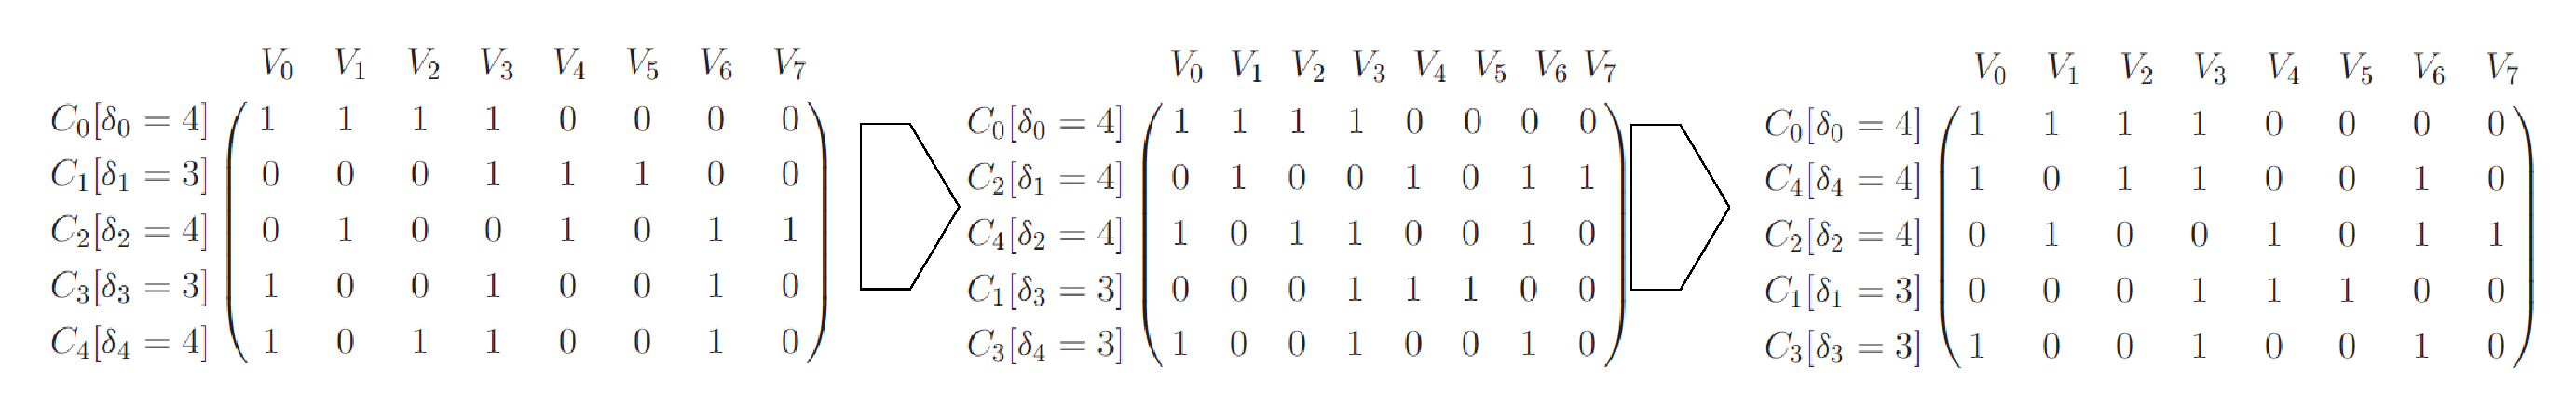
\includegraphics[width = \textwidth]{matrix.pdf}
	\caption{CN Computation Reordering}
\end{figure}
空间占用情况:
\begin{equation}
	\Delta = q \times n + q \times m + 2 \times m.
\end{equation}
\subsection{其他}
1. 预先计算好En地址;\\
2. 使用最新的指令集;\\
3. 多核计算。

%===========第二节=================
\section{代码学习}
\begin{figure}[H]
	\centering
	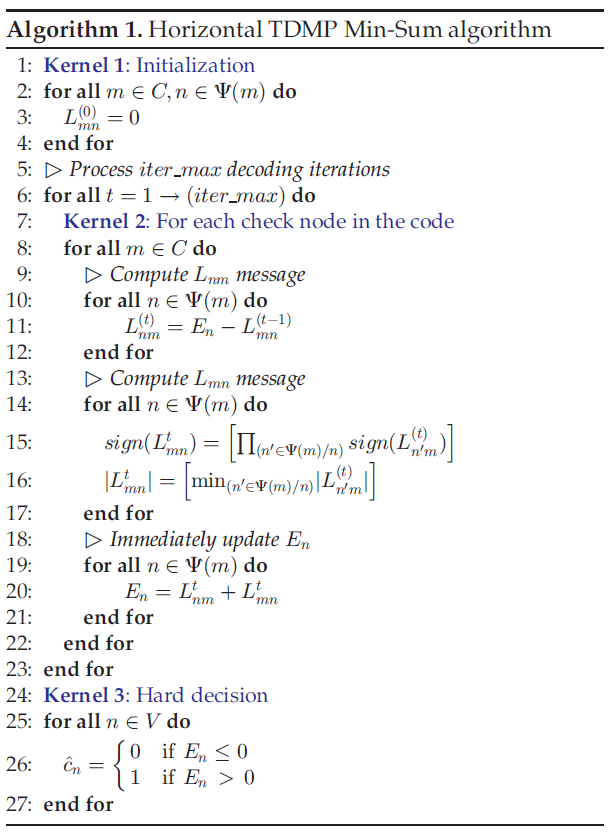
\includegraphics[width = .6\textwidth]{alg.png}
\end{figure}

%===========第三节=================
\section{存在问题}
\begin{figure}[H]
	\centering
	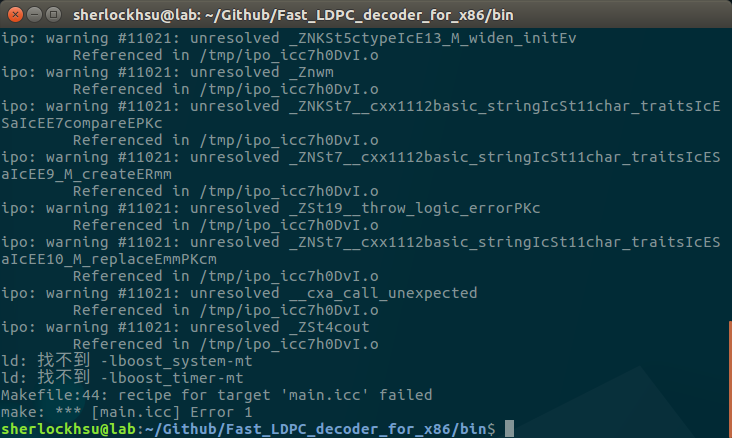
\includegraphics[width = .8\textwidth]{err.png}
\end{figure}

%===========第四节=================
% \section{仍存在问题}


%===========下周计划=================
\section{下阶段计划}
1. 使程序正常运行;\\
2. 尝试与原仿真程序结合。

\end{document}
%%%%%%%%%%%%%%%%%%%%%%%这是正文部分的结束%%%%%%%%%%%%